\subsection{Реляционная алгебра. Соединения}

\subsubsection{Полное соединение}

\begin{definition}
	\textit{Полным соединением} называется декартово произведение двух отношений. Заголовком
	является объединение заголовков, а телом -- декартово произведение тел отношений.
\end{definition}

\begin{remark}
	Необходимым условием выполнимости этой операции является отсутствие общих имен атрибутов. При
	желании, этого можно добиться операцией переименования (см. \ref{def-rename}).
\end{remark}

На рисунке \ref{full-join-ex} приведен пример полного соединения.

\begin{figure}[H]
	\centering
	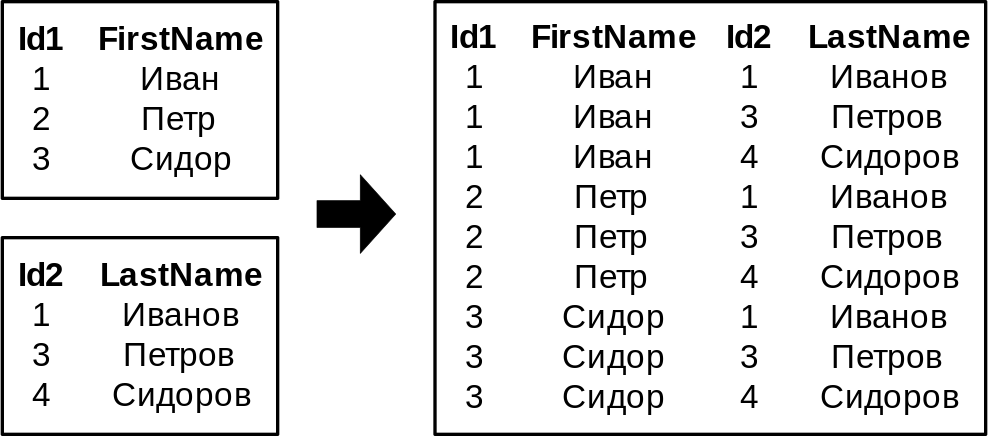
\includegraphics[width=0.8\textwidth]{../assets/kgeorgiy/relalgebra/Join_Full_2.svg.png}
	\caption{Пример полного соединения}
	\label{full-join-ex}
\end{figure}

\subsubsection{Естественное соединение}\label{nat-join-def}

\begin{definition}
	\textit{Естественным соединением} называется операция, при которой у двух отношений соединяются
	кортежи, имеющие равные значения атрибутов с одинаковыми именами. Обозначается
	$R_1 \bowtie R_2$. Заголовком является объединение заголовков.
\end{definition}

\begin{remark}
	При отсутствии общих атрибутов в заголовках отношений, естественное соединение эквивалентно
	полному.
\end{remark}

На рисунке \ref{nat-join-ex} приведен пример естественного соединения.

\begin{figure}[H]
	\centering
	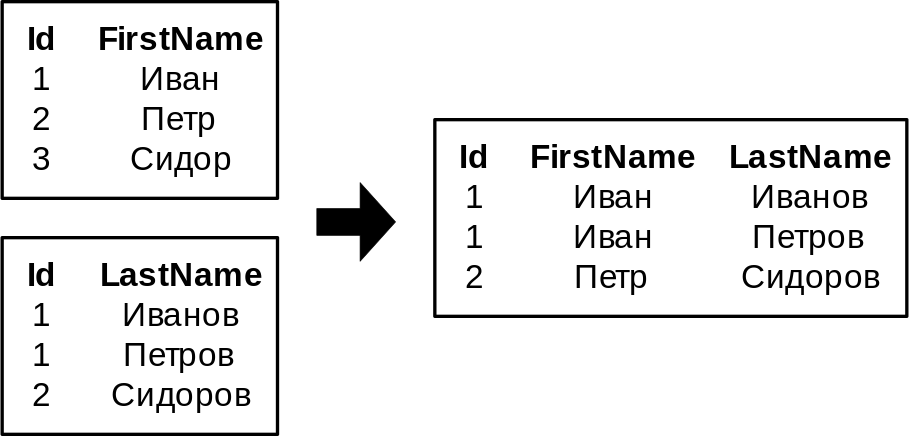
\includegraphics[width=0.8\textwidth]{../assets/kgeorgiy/relalgebra/Join_Natural_2.svg.png}
	\caption{Пример естественного соединения}
	\label{nat-join-ex}
\end{figure}

\paragraph{Размер естественного соединения}

Нетрудно понять, какой минимальный и максимальный размер естественного соединения может получится:
\[
	0 \leqslant \left|R_1 \bowtie R_2 \right| \leqslant |R_1| \times |R_2|.
\] Нижняя оценка достигается при отсутствии равных атрибутов, верхняя -- при
отсутствии общих атрибутов в заголовке.

\subsubsection{Внешнее соединение}

\begin{definition}
	\textit{Внешнее соединение} похоже на естественное (см. \ref{nat-join-def}), только оно
	дополнительно сохраняет те кортежи, для которых нет соответствующих во втором отношении. Вместо
	соответствующего берется пустой кортеж. Заголовком все так же является объединение заголовков.
	Обозначение: $R_1 \oujoin R_2$.
\end{definition}

На рисунке \ref{outer-join-ex} приведен пример внешнего соединения.

\begin{figure}[H]
	\centering
	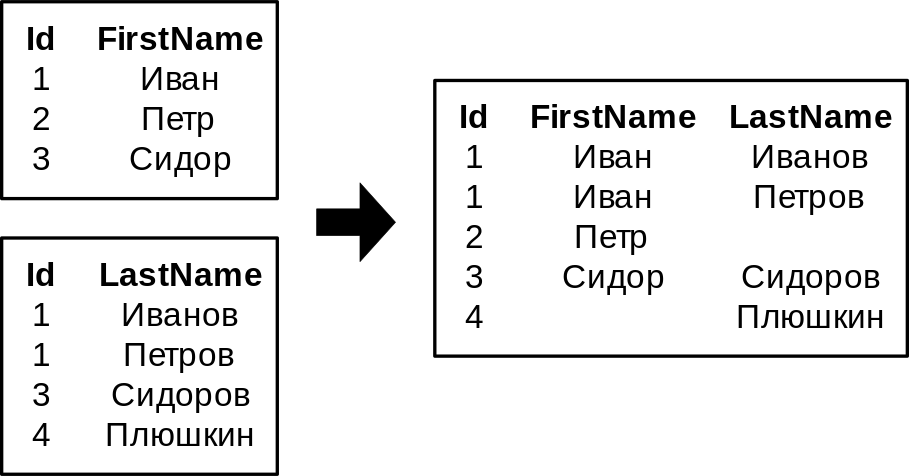
\includegraphics[width=0.8\textwidth]{../assets/kgeorgiy/relalgebra/Join_Outer_2.svg.png}
	\caption{Пример внешнего соединения}
	\label{outer-join-ex}
\end{figure}

\subsubsection{Левое и правое соединения}

\begin{definition}
	\textit{Левое соединение} похоже на естественное (см. \ref{nat-join-def}), только оно
	дополнительно сохраняет те кортежи левого отношения, для которых нет соответствующих в правом
	отношении. Вместо соответствующего берется пустой кортеж. Заголовком все так же является
	объединение заголовков. Обозначение: $R_1 \ljoin R_2$. Правое определяется симметрично и
	обозначается $R_1 \rjoin R_2$.
\end{definition}

\begin{remark}
	\[
		R_1 \ljoin R_2 \equiv (R_1 \njoin R_2) \cup (R_1 \setminus \pi_{R_1}(R_1 \njoin R_2)),
	\]
	\[
		R_1 \rjoin R_2 \equiv (R_1 \njoin R_2) \cup (R_2 \setminus \pi_{R_2}(R_1 \njoin R_2)).
	\]
	Кроме того, через левое и правое соединения можно выразить внешнее: \[
		R_1 \oujoin R_2 \equiv (R_1 \ljoin R_2) \cup (R_1 \rjoin R_2).
	\]
\end{remark}

На рисунке \ref{lr-join-ex} приведены примеры косых соединений $R_1 \ljoin R_2$ и
$R_1 \rjoin R_2$.

\begin{figure}[H]
	\centering
	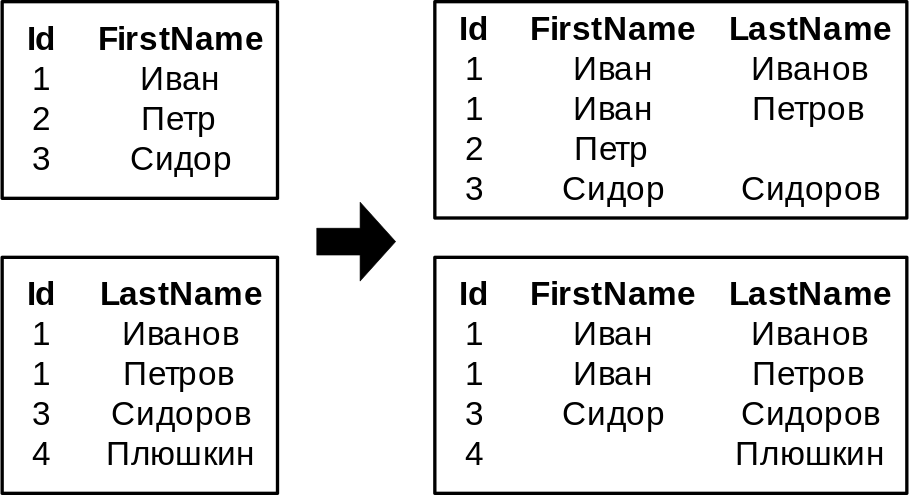
\includegraphics[width=0.8\textwidth]{../assets/kgeorgiy/relalgebra/Join_LeftRight_2.svg.png}
	\caption{Примеры косых соединений}
	\label{lr-join-ex}
\end{figure}

\subsubsection{Полусоединения}

\begin{definition}
	\textit{Левым (правым) полусоединением} называется следующее отношение: $R_1 \lhjoin R_2 \equiv \pi_{R_1}(R_1 \njoin R_2)$
	($R_1 \rhjoin R_2 \equiv \pi_{R_2}(R_1 \njoin R_2)$). Иначе говоря, это отношение, состоящее из
	строк левого (правого) отношения, для которых есть соответствующие строки в правом (левом).
\end{definition}

\begin{remark}
	\enewline
	\begin{itemize}
		\item $R_1 \ljoin R_2 = (R_1 \njoin R_2) \cup (R_1 \setminus R_1 \lhjoin R_2)$.
		\item $R_1 \rjoin R_2 = (R_1 \njoin R_2) \cup (R_2 \setminus R_1 \rhjoin R_2)$.
	\end{itemize}
\end{remark}

На рисунке \ref{lrh-join-ex} приведены примеры полусоединений $R_1 \lhjoin R_2$ и
$R_1 \rhjoin R_2$.

\begin{figure}[H]
	\centering
	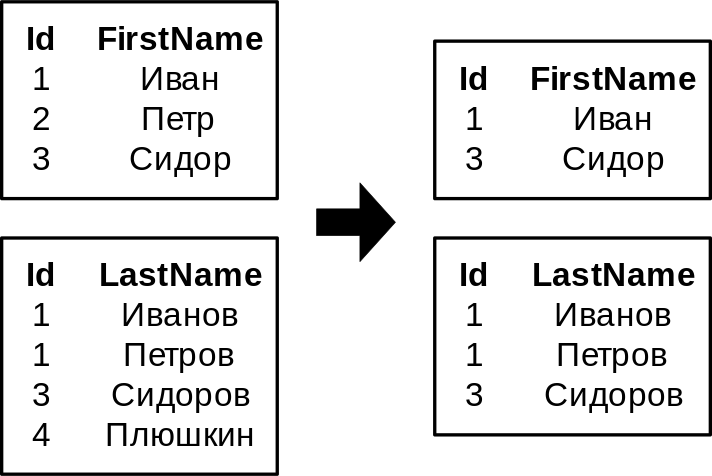
\includegraphics[width=0.8\textwidth]{../assets/kgeorgiy/relalgebra/Join_Semi_2.svg.png}
	\caption{Примеры полусоединений}
	\label{lrh-join-ex}
\end{figure}

\subsubsection{Условные соединения}

\begin{definition}
	Возьмем любое соединение и наложим на него дополнительное условие $\theta$. Получится
	соответствующее условное соединение. Имеется в виду, что нужно отфильтровать результат соединения.
	Однако, не всегда это возможно. Покажем на нескольких примерах, как это должно выглядеть.
	\begin{itemize}
		\item $R_1 \njoin_\theta R_2 = \sigma_\theta(R_1 \njoin R_2)$.
		\item $R_1 \ljoin_\theta R_2 = J \cup (R_1 \setminus \pi_{R_1}(J)),~ J = \sigma_\theta(R_1 \njoin R_2)$.
		\item $R_1 \rjoin_\theta R_2 = J \cup (R_2 \setminus \pi_{R_2}(J)),~ J = \sigma_\theta(R_1 \njoin R_2)$.
		\item $R_1 \oujoin_\theta R_2 = (R_1 \ljoin_\theta R_2) \cup (R_1 \rjoin_\theta R_2)$.
	\end{itemize}
\end{definition}

На рисунке \ref{theta-join-ex} приведен пример левого условного соединения
$R_1 \ljoin_{|FirstName| + 2 < |LastName|} R_2$.

\begin{figure}[H]
	\centering
	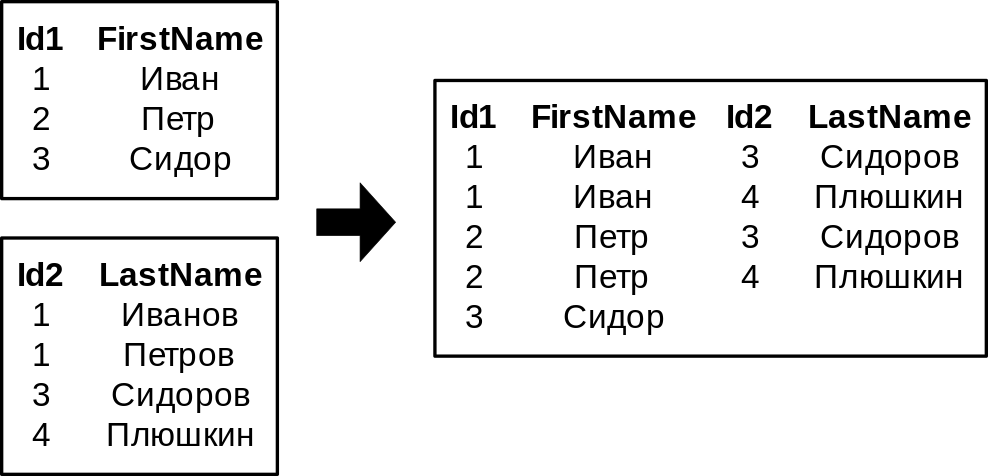
\includegraphics[width=0.8\textwidth]{../assets/kgeorgiy/relalgebra/Join_LeftTheta_2.svg.png}
	\caption{Пример левого условного соединения}
	\label{theta-join-ex}
\end{figure}

